\chapter{Design Considerations for Interactive Tag Cloud Visualisation}
\label{chap:tagcloud}
\ifpdf
    \graphicspath{{Chapters/TagCloudDesign/TagCloudDesignFigs/PNG/}{Chapters/TagCloudDesign/TagCloudDesignFigs/PDF/}{Chapters/TagCloudDesign/TagCloudDesignFigs/}}
\else
    \graphicspath{{Chapters/TagCloudDesign/TagCloudDesignFigs/EPS/}{Chapters/TagCloudDesign/TagCloudDesignFigs/}}
\fi


Tag clouds have been used to visualise books, speeches, and other text through online tools such as Wordle\footnote{\url{http://wordle.net/}}, TagCrowd\footnote{\url{http://tagcrowd.com/}} and Manyeyes\footnote{\url{http://www-958.ibm.com/software/analytics/manyeyes/}}. While these tools easily create aesthetically pleasing clouds for users, their full potential for information visualisation is unrealised. As we saw in \S\ref{sect:tagcloudsinsoftware}, those few tools which have sought to apply the tag cloud paradigm to multi-variate data, have failed to take into consideration certain aspects (such as long identifiers) which have consequently proved problematic. In this chapter we develop design considerations for an interactive tag cloud visualisation system by reviewing design principles, guidelines, and research in general information and tag cloud visualisation. Furthermore, we present a set of task types that should be supported in order to enable data exploration. These task types are generated from analysing the challenges in visualising software and multi-variate data, as well as the capabilities of tag clouds. The task types and design considerations are used to inform the design of our interactive tag cloud visualisation system `Taggle', presented in Chapter~\ref{chap:taggle}.

\section{Visual variables}\label{sect:visualvariables}

Tools such as Wordle or TagCrowd generate tag clouds which display word frequency counts through the font size of individual tags. Other visual properties (such as colour, ordering and typeface styles) are generally ignored or used in a decorative fashion. We contend that these alternate visual properties available in tag clouds can and should be used to represent other data variables or reinforce mappings. With these visual properties representing data, a tag cloud can support users in tasks such as gisting, searching and knowledge extraction. In the creation of our interactive tag cloud visualisation system Taggle, consideration had to be given to the amount of influence on user perception for each visual variable, as well as their individual properties which affected suitability of being mapped to data. 

Due to the textual nature of tag cloud visualisation, many visual properties in tag clouds relate to font characteristics. Phrase or keyword emphasis in tag clouds are manipulated via typographical techniques. These can be applied with various design principles \citep[such as those outlined in the seminal manual ``The elements of typographical style''][]{bringhurst01}. Tag emphasis in clouds (for individual data points) may be created through manipulation of variables such as size, colour, font family or style. Visual properties of tag clouds that may influence perception can be seen in Table~\vref{table:visualproperties}, although not all properties may be suitable to map to data variables. An example of data mapped to some of these properties may be seen in Figure~\vref{fig:tagmapping}.

\begin{table*}
\centering
\caption{\textit{Visual properties that may influence perception in tag clouds}}
\begin{tabular}{|p{4cm}|p{8cm}|} \hline
\textbf{Visual Property}&\textbf{Types}\\ \hline
Layout & typewriter\par spiral\\ \hline
Order & alphabetical\par semantic\par random\\ \hline
Tag length & variable number of characters\par equal number of characters\\ \hline
Tag position & top left quadrant\par top right quadrant\par bottom left quadrant\par bottom right quadrant\\ \hline
Font size & \\ \hline
Font family& Serif vs Sans-serif\par Arial\par Times New Roman \\ \hline
Font colour & hue\par saturation\par value \\ \hline
Background colour & hue\par saturation\par value \\ \hline
Font style & bold vs normal\par italics vs normal\par all capitals vs mixed case\par underline vs normal   \\ 
\hline\end{tabular}
\label{table:visualproperties}
\end{table*}

\begin{figure}[!htb]
	\centering
	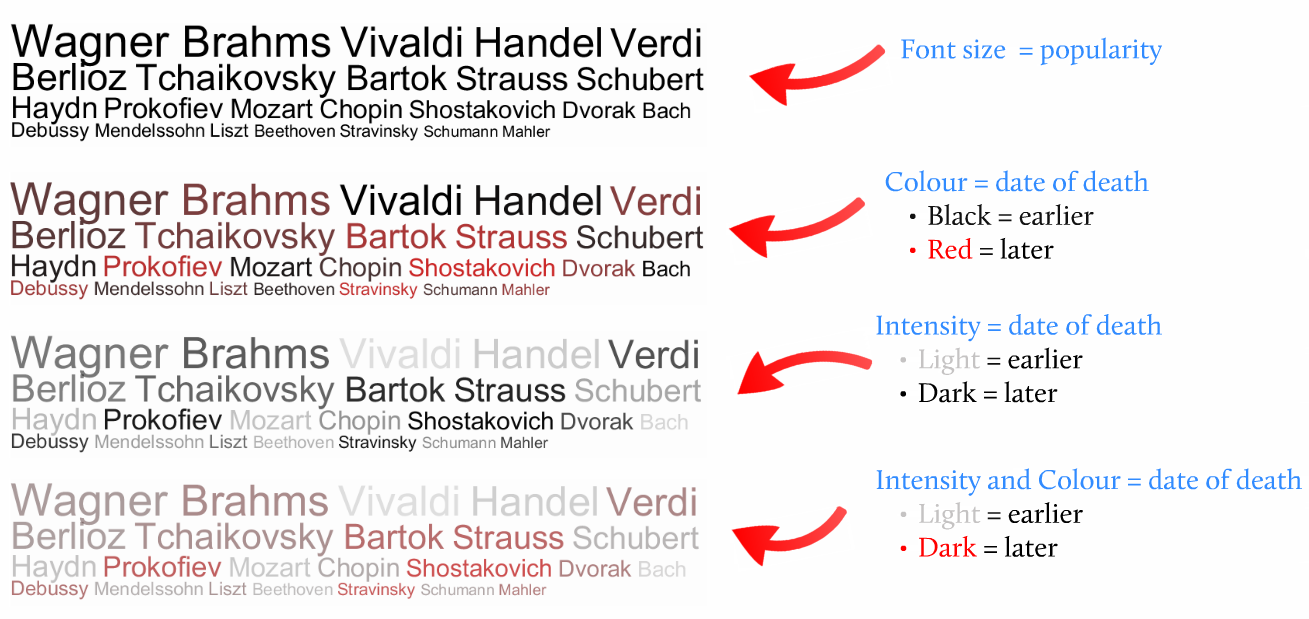
\includegraphics[scale=0.40]{mapping.png}
	\caption{\textit{Popularity ranking of composers: mapping of artificial data to tag cloud visual properties (tag clouds generated by Taggle).}}
	\label{fig:tagmapping}
\end{figure}

\subsection{Visual mapping} 

The term `visual variables', as introduced by \citet{bertin83} in the ``Semiology of Graphics'', refers to a specified set of symbols that can be applied to data in order to translate information. This process of mapping data to visual properties is called `visual mapping'. The visual variables are defined as position, size, shape, value, colour (hue), orientation, and texture. Choosing a particular variable to map to data depends on an analysis of the characteristics of the variable. Each variable's characteristics are defined from the following list of perceptual approaches:

\begin{itemize}
	\item Selective: If a data point can easily be selected as being different from the other data points.
	\item Associative: If multiple data points can be perceived as being similar.
 	\item Quantitative: If data points can be perceived as being proportional to one another.
 	\item Ordered: If data points can be interpreted in an order.
	%\item Length: How many values a variable can meaningfully contain.
\end{itemize}

When creating a data visualisation, it is important to know and appropriately use the characteristics of a visual variable. In the following subsections the effects on user perception for each tag cloud visual variable is discussed with respect to Bertin's perceptual approaches, other design guidelines and tag cloud research. Likely suitability for data mapping within a tag cloud is determined.

\subsection{Layout and order}\label{sub:layout}

Layouts of tags within a tag cloud are generally based on either a typewriter style (tags arranged from left to right, and top to bottom), or arranged in a spiral pattern. Relevant ordering of the tags within the tag cloud layout (within constraints imposed by such things as window shape) is important for users of the visualisation tools when applying search and locate tasks. Previous research has indicated alphabetical ordering of tags is generally preferable to random or semantically clustered layouts when searching for a named tag within a tag cloud, although semantic clustering can provide improvements over random arrangements \citep[][]{halvey07, schrammel09}. 

However, the ordering property is also suitable for search and locate tasks using variables not related to the tag text. For instance, using the ordering property to locate tags with maximum or minimum values of a variable, in Figure~\vref{fig:datasets1} once it is understood that the ordering of the tags is related to the popularity of a name within the USA, it is easily found that the top three most popular boys names in the US are Michael, Christopher and Matthew. Likewise, in Figure~\vref{fig:background}, it can easily be seen that Bahamas had the greatest number of gold medals in the Olympic medal ranking based on a per-capita ranking system.

\begin{itemize}
	\item \emph{\textbf{Tag order:} Visual property tag order is suitable for mapping to data fields}
\end{itemize}

\subsection{Tag length and position} 

Longer tag lengths have been shown to have an effect on user perception of tag importance \citep{bateman08}. Tags placed in the upper left quadrant of a tag cloud are found more quickly \citep{bateman08} and are also better recalled \citep{rivadeneira07}. Analysis of eye-tracking data has shown the upper left quadrant of a tag cloud receives the most attention \citep[][]{lohmann09, schrammel09b}. It is possible the upper left quadrant dominance is due to western language reading patterns. Due to this quadrant prominence, tag position is a particularly appropriate mapping for search and locate tasks through use of the ordering property (\S\ref{sub:layout}) when tag clouds are arranged in a typewriter fashion. 

\begin{itemize}
	\item \emph{\textbf{Equal length tag identifiers:} It should be possible to set the length of the tag identifiers to an equal length to minimise effects on user perception}
\end{itemize}

\subsection{Font size} \label{sect:fontsize}

Text size manipulation can be a very effective way of creating emphasis. Empirical research on tag cloud visual properties has identified size as having a significant effect on user perception \citep[for example][]{lohmann09, bateman08, halvey07}. This means large font sized tags are found more quickly than small font sized tags. For example, in Figure~\vref{fig:datasets2} user names `pam120', `kfc172' or `gey66' can immediately be located in the tag cloud due to their prominence from a comparatively large font size.

The size visual variable is selective, associative, ordered, and quantitative \citep{bertin83}, although care must be taken when using size quantitatively, as changes in size from volume or area may be difficult to interpret \citep{carpendale03}. According to \citep{bateman08, schrammel09b} font size can be accurately compared in a tag cloud.

Because of canvas and screen boundaries, there are limitations in the maximum font sizes which can be displayed within a tag cloud. With regard to minimum font sizes, guidelines based on reading performance research state a 9pt font limit for web pages or screen media \citep[pg 107, chap 11:8][]{usability06}.
 
For data mapping purposes, font size is an appropriate visual variable candidate for mapping to data variables in a tag cloud. Careful attention should be paid to minimum font sizes for reading ease. 

\begin{itemize}
	\item \emph{\textbf{Font size:} Visual property tag order is suitable for mapping to data fields}	
	\item \emph{\textbf{Constrained font sizes:} Font size should be constrained to greater than 9pt, and a suitable maximum font size according to canvas and screen boundaries}
	\item \emph{\textbf{Comparable tags:} Tags should be able to be compared by moving closer together to assist quantitative comparisons}
\end{itemize}

\subsection{Font Family}   

Typographical characteristics such as font family were not mentioned by \citet{bertin83}. The shape visual variable, which is the most closely related variable mentioned, is not perceived as an especially effective variable. According to \citet{carpendale03}, shape may be selective and associative, providing there are minimal data points or minimal shape variations. 

In tag cloud research, \citet{waldner13} found text orientation and shape modifications performed significantly worse than colour coding for distinguishing tag categories. Many users also perceived rotated tags as unstructured and unattractive. Shape differences caused by serifs or font styles were hard to detect in controlled experiments using the Helvetica font style. It is also possible that manipulation of font family may alter user perception of other font styles used as a mapping variable, such as bold or italic. It does not seem that font family would be an effective data mapping visual property within a tag cloud. 

Research shows that reading speed is best when users are presented with familiar fonts such as Times New Roman, Arial or Helvetica  \citep[pg 106, chap 11:7][]{usability06}. These fonts may therefore be preferable in a tag cloud for reading accuracy.

\begin{itemize}
	\item \emph{\textbf{Font family:} Visual property tag order is not suitable for mapping to data fields}	
	\item \emph{\textbf{Familiar fonts:} For reading accuracy, fonts should be familiar such as Times New Roman, Arial or Helvetica}	
\end{itemize}

\subsection{Font colour}\label{sect:fontcolour}

In a study of the effectiveness of textual retinal properties in tag clouds, \citet{waldner13} found that after font size, colour (both as text colour or as the tag's background colour) was the most effective visual text variable for encoding nominal and ordinal data. On the other hand, transparency was disliked by users and lead to inaccurate results when determining tags of relevance. \citet{bateman08} found that colour intensity (saturation/transparency) had a relatively good influence on user perception, although not as strong as font size. 

\citet{preston10} investigated the effectiveness of typographical emphasis techniques (such as colour, bold and italics) on computer presentation software. They found that use of colour in font emphasis techniques generally elicited significantly faster response times identifying  text than achromatic techniques such as bold and italic, provided a suitable colour contrast was given.

Colour value has properties selective, associative and ordering \citep{bertin83}, whereas colour hue has only selective and associative properties and cannot be perceived by a viewer in an ordered fashion. Value may be considered to be quantitative also, in that lighter value colours are perceived to be related to smaller numbers and darker colour values to higher numbers, but actual quantitative comparison can be difficult (for example perceiving one shade of colour as being three times darker than another shade). 

Ware's information visualisation guidelines advise not using more than ten colours for coding symbols (especially if the symbols are to be used against a variety of backgrounds) \citep[pg 124, chap 4, G4.15][]{ware04}. Ware also recommends twelve specific colours for use in coding: red, green, yellow, black, blue, white, pink, cyan, grey, orange, brown, and purple \citep[pg 126, chap 4, G4.18][]{ware04}.

For data mapping purposes, it may be more useful to consider colour value and saturation as being aligned to a transparency mapping often employed as a visual property in tag clouds. Both hue and transparency are appropriate candidates for mapping to data variables in a tag cloud. Consideration must be given to colour choice, contrasts and quantitative mapping.

\begin{itemize}
	\item \emph{\textbf{Colour hue:} Visual property colour hue is suitable for mapping to data fields}	
	\item \emph{\textbf{Colour transparency:} Visual property colour transparency is suitable for mapping to data fields}	
	\item \emph{\textbf{Colour selection:} Colour codes should be taken from Ware's  colour code recommendations (red, green, yellow, black, blue, white, pink, cyan, grey, orange, brown, and purple)}	
\end{itemize}

\subsection{Background Colour}\label{sect:backgroundcolour}

Background colour is an appropriate data mapping visual variable as an alternative to font colour. As discussed in \S\ref{sect:fontcolour}, \citet{preston10} found that use of colour in typographical emphasis techniques elicited faster response times identifying emphasised text than achromatic techniques. This performance improvement was providing a suitable colour contrast was given (such as red, green or blue on a white background). Consideration of text colour against background must be given during colour selection of visual mappings within a tag cloud. 

It is possible to manipulate background colour on an individual tag. This could have two possible benefits 1) it allows grouping together of multiple keywords or phrases, and 2) mapping the colour to the background behind the tag may have a greater effect on user perception than mapping the colour to the text. This is because the area of the background behind the tag is greater than the area of the font text itself and in general, the larger the area that is colour coded, the more easily colours can be distinguished \citep[pg 125, chap 4][]{ware04}. Colour coding in the tag background has been found to support more accurate estimation of relevant tags than font colour \citep{waldner13}.

Chapter~\ref{chap:eval} details empirical research conducted which included investigation of the benefits of background colour manipulation in tag clouds. For an example of text and background colour in a tag cloud see Figure~\vref{fig:background}, which shows Olympic medal rankings using both gold first and per-capita ranking systems. Countries which have more than one word in their name are more easily distinguished using background colour mapping.

\begin{figure}[!htb]
\begin{subfigure}{\textwidth}
	\centering
	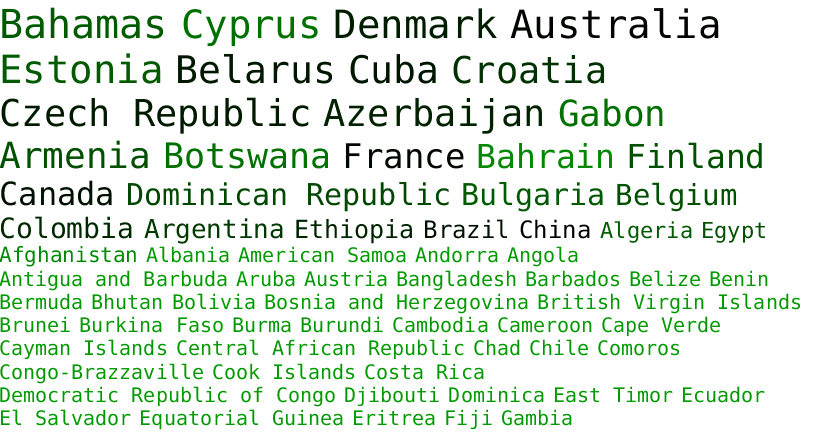
\includegraphics[scale=0.50]{foregroundex.png}
	\label{fig:foregroundsub}
	\caption{\textit{Font colour}}
\end{subfigure}
\begin{subfigure}{\textwidth}
  \centering
  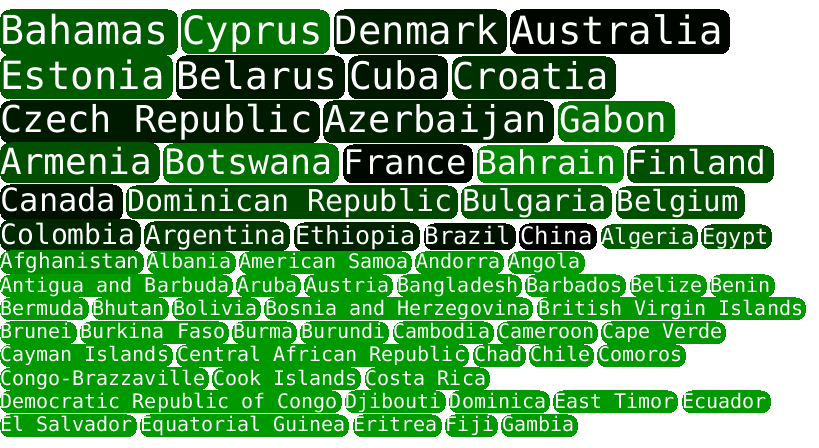
\includegraphics[scale=0.50]{backgroundex.png}
  \label{fig:backgroundsub}
  \caption{\textit{Background colour}}
\end{subfigure}
  \caption{\textit{Olympic medal rankings: size and order are mapped to per-capita ranking system. Colour is mapped to standard (gold first) ranking system.}}
  \label{fig:background}
\end{figure}

\begin{itemize}
	\item \emph{\textbf{Colour background:} Visual property colour background is suitable for mapping to data fields}	
	\item \emph{\textbf{Colour contrasts:} Strongly contrasting colour schemes should be selected such as red, green or blue on a white background}	
\end{itemize}

\subsection{Font Style}   

Font styles or typography in general were not included in Bertin's visual variables \citet{bertin83}. \citet{bateman08}'s exploration of the effects of various properties and characteristics of text in tag clouds found that weight (bold style) had a consistently strong influence on user perception. A comprehensive study on the effectiveness of emphasis techniques in presentations by \citet{preston10} found bold text performed well with black text on a white background but not with white text on black.  \citet{preston10} found capitals to be the most effective of the achromatic emphasis techniques, although all four techniques (capitals, bold, italics and underline) did not perform as well as the chromatic techniques (use of colour).  Underline and italic emphasis techniques were consistently the least effective means of emphasising text. 

Font styles bold and underline are considered more effective as text emphasis than italic or underline. The number of differing values that these typographical styles may show is only two (underline on, underline off --- bold on, bold off) so is likely not worth including as a data mapping variable in a tag cloud. 

\begin{itemize}
	\item \emph{\textbf{Font styles:} Visual property font styles are not considered suitable for mapping to data fields}	
\end{itemize}

\section{Challenges in software visualisation}\label{sect:challenges}

In the software engineering domain, quality metric data distributions are typically heavily skewed and may contain outliers (see Figure~\vref{fig:distributions}). Unlike some other disciplines, where outlying data points may be discarded or ignored, in software engineering these outliers are potentially the most interesting and should be investigated further as potential candidates for refactoring. 

\begin{figure}[!htb]
   	\centering
  	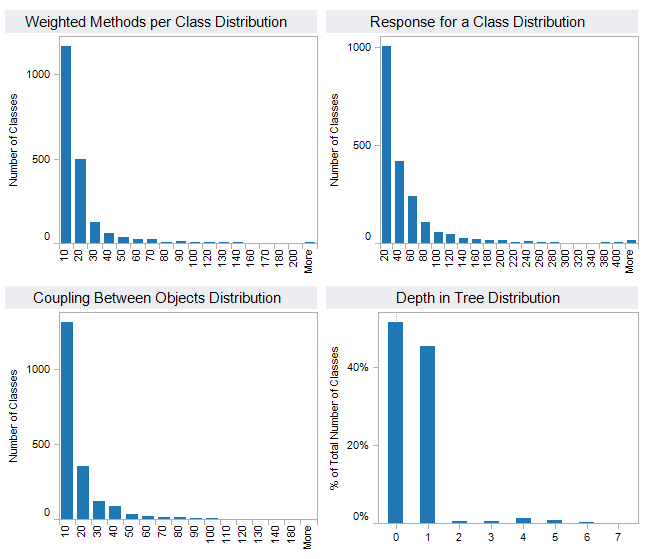
\includegraphics[scale=0.70]{distributions.png}	
	\caption{\textit{Distribution of Chidamber and Kemerer metrics for open source project AspectJ (calculated by CKJM toolkit)}}
	\label{fig:distributions}
\end{figure}

In the software visualisation domain, and many datasets in general, there may be a large numbers of data points which cover large ranges of values. There are also various size constraints to be considered such as the size of the screen, symbols, fonts or other identifiers. One general information visualisation technique for management of this problem is to incorporate interactivity into the visualisation, first providing the user with an overview, then zooming and filtering, and obtaining the information details on demand. This principle is called the ``Information Seeking Mantra'' and was introduced by \citet{schneiderman96}. Another technique is to display an overview of data but allow detailed information to be displayed simultaneously (also known as focus+context) such as with fish-eye. 

There is a variety of textual information contained in many general datasets, and software datasets are no exception (for example class, method or package names, bug categories and rankings, and agile stories and tasks). Text is problematic for some multi-variate visualisation techniques (such as scatterplots or treemaps) due to space limitations. No one visualisation method or technique may provide a good balance for all considerations for a software engineering dataset and a combination of techniques may be necessary, using whichever method is most effective for a particular context.

\section{Datasets for the tag cloud technique}\label{sect:datasets}

One of the benefits of tag cloud visualisation is that data point textual identifiers (such as names) are an integral part of the graphic, meaning that users don't have to navigate into the visualisation to find important information. With this in mind, the sort of dataset that would be optimal to display in a tag cloud is one which includes modest amounts of textual information. Many datasets include this sort of information, in the form of names, labels or identifiers. In a general capacity, example datasets that might be used include names of people, brand names or marketing data, company financial information, stock market or foreign exchanges, country statistics, animal endangerment ratings, sporting events, file and folder names in a computer, and so on. Software engineering datasets also contain this sort of data such as class, method or package names, bug categories and rankings, and agile stories and tasks. See Figures~\ref{fig:datasets1} and \ref{fig:datasets2} for examples of a general and software related dataset.

\begin{figure}[!htb]
	\centering
	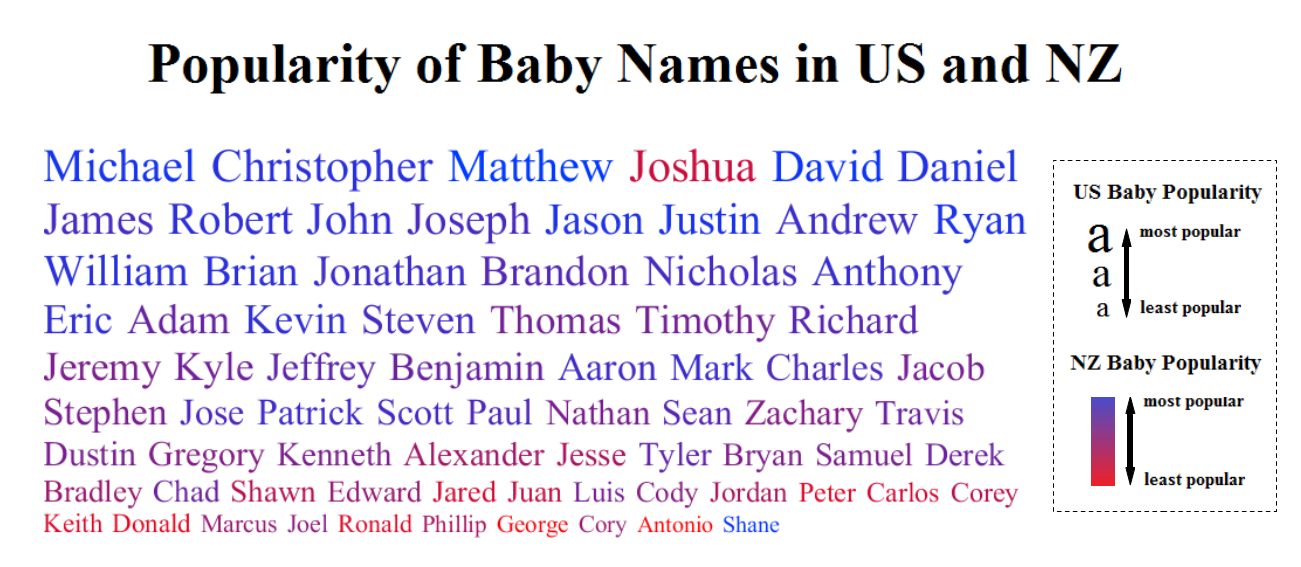
\includegraphics[scale=0.35]{babynames.png}
	\label{fig:babynames}
	\caption{\emph{Popularity of baby names}}
      \label{fig:datasets1}
\end{figure}

\begin{figure}[!htb]
  \centering
  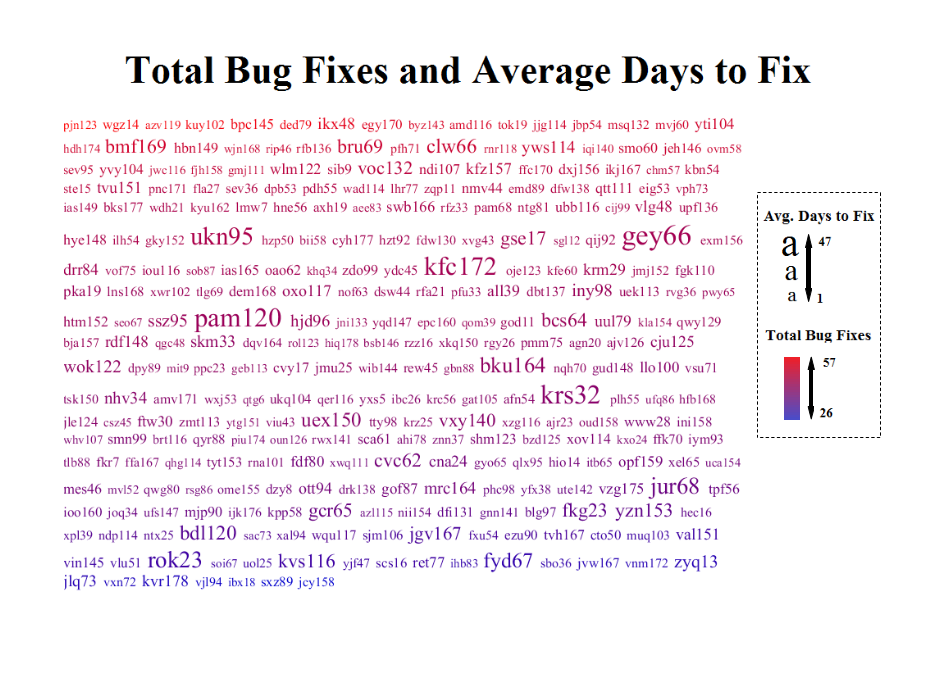
\includegraphics[scale=0.50]{buglist.png}
  \label{fig:buglist}
  \caption{\emph{Bug fixes for each user}}
  \label{fig:datasets2}
\end{figure}

Much of the important textual data contained in these sorts of datasets is a phrase or collection of words rather than just one word. Also, many datasets containing some sort of label or identifier utilise many characters --- such as a fully qualified file or class name. It is important to note that multiple word phrases and lengthy label names can waste valuable real estate in the visualisation. There are two possible issues with this 1) it may have the effect of the data point appearing to have more importance than it actually does due to the increased prominence of the text, and 2) with multiple word tags it may be difficult to distinguish the boundaries between data points (this can be seen in Figure~\vref{fig:birds}).

\begin{figure}[!htb]
	\centering
	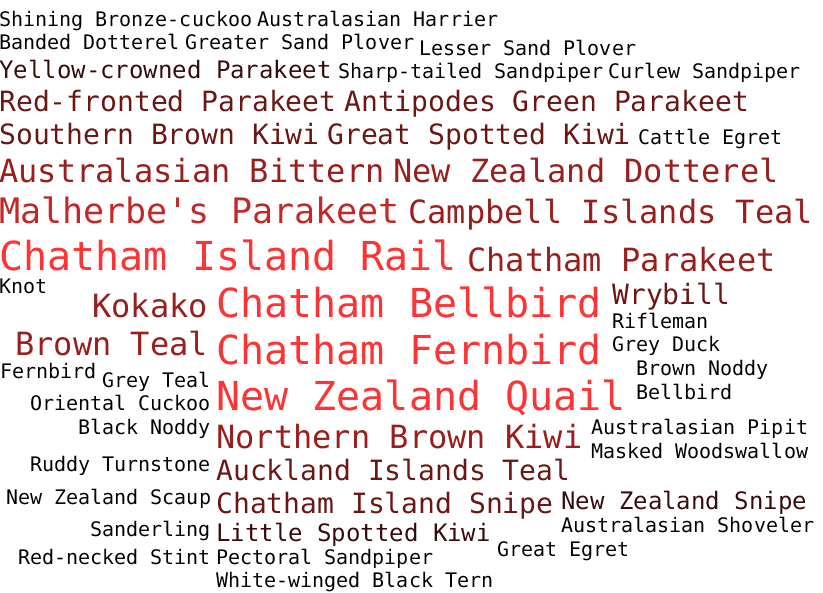
\includegraphics[scale=0.50]{birds.png}
	\caption{\emph{Endangered species ranking for NZ birds}}
	\label{fig:birds}
\end{figure}

\begin{itemize}
	\item \emph{\textbf{Textual datasets:} Optimal datasets contain textual identifiers such as class names or stories}
	\item \emph{\textbf{Filterable tag phrases:} Multiple words waste valuable real estate in a visualisation, so should be filterable}
	\item \emph{\textbf{Establish tag boundaries:} Boundaries between tags with multiple words should be clearly established}
\end{itemize}

\section{Task types to enable data exploration in a tag cloud}\label{sect:tasktypes}

It was suggested by \citet{rivadeneira07} in early empirical work, that the task set supported by tag clouds includes searching, browsing, impression forming and recognition/matching. Evidence exists that suggests tag clouds can provide improvements for summarising descriptive information (overviews) and also that they may be useful as a descriptive supplement for traditional search interfaces \citep{kuo07, sinclair08}. However, research has compared tag clouds negatively to tables or lists for search and locate tasks \citep[such as][]{oosterman10, halvey07, kuo07, rivadeneira07}. These experiments which report sub-optimal results for tag clouds required searching for or locating textual tag names and do not ask users to complete a visual search using additional features such as colour. (See Chapters~\ref{chap:exp1} and  \ref{chap:exp2} which investigate the possibility of the use of tag background colour or dual visual feature mapping improving user performance in a visual search.) Furthermore, we believe that more complex datasets (such as those with multiple data variables and intricate relationships between records) and other domain-specific factors, add more substance than the simplistic search and locate experiments might suggest. 

We have identified an appropriate set of tasks shown in Table~\vref{tab:taskset} which match the potential capabilities of tag clouds to tasks that are useful in software engineering (and also have a wider application in multi-variate data analysis). For categorisation purposes these can be further assigned to task types associated with data mining.

\begin{table}
\centering
\caption{\textit{Tasks}}
\begin{tabular}{|p{8cm}|p{3cm}|} \hline
 \textbf{Task Description} & \textbf{Task Type} \\ \hline
Identify similar characteristics of data & Clustering \\
Identify data distribution & Summarising \\
Identify data correlations & Associative \\
Detect outliers in a correlation & Summarising \\
Finding minimum/maximum values & Classifying \\
Comparison of data elements  & Classifying\\\hline
\end{tabular}
\label{tab:taskset}
\end{table}

As an example of how tag clouds may be used to complete the associative task of identify correlations between variable, see Figure~\vref{fig:tagcorrelation} which shows (artificially composited) composer popularity against the date of death. We can see that modern composers (who died later) are more popular than composers who died earlier such as those from the Classical or Baroque period. In Figure~\vref{fig:datasets2} we can use the tag cloud font size to establish a general data distribution (summarising task). Most user names in the tag cloud are very small with only a few larger names, therefore we can hypothesise that most users take a comparatively lower number of days to complete bug fixes.

\begin{figure}[!htb]
	\centering
	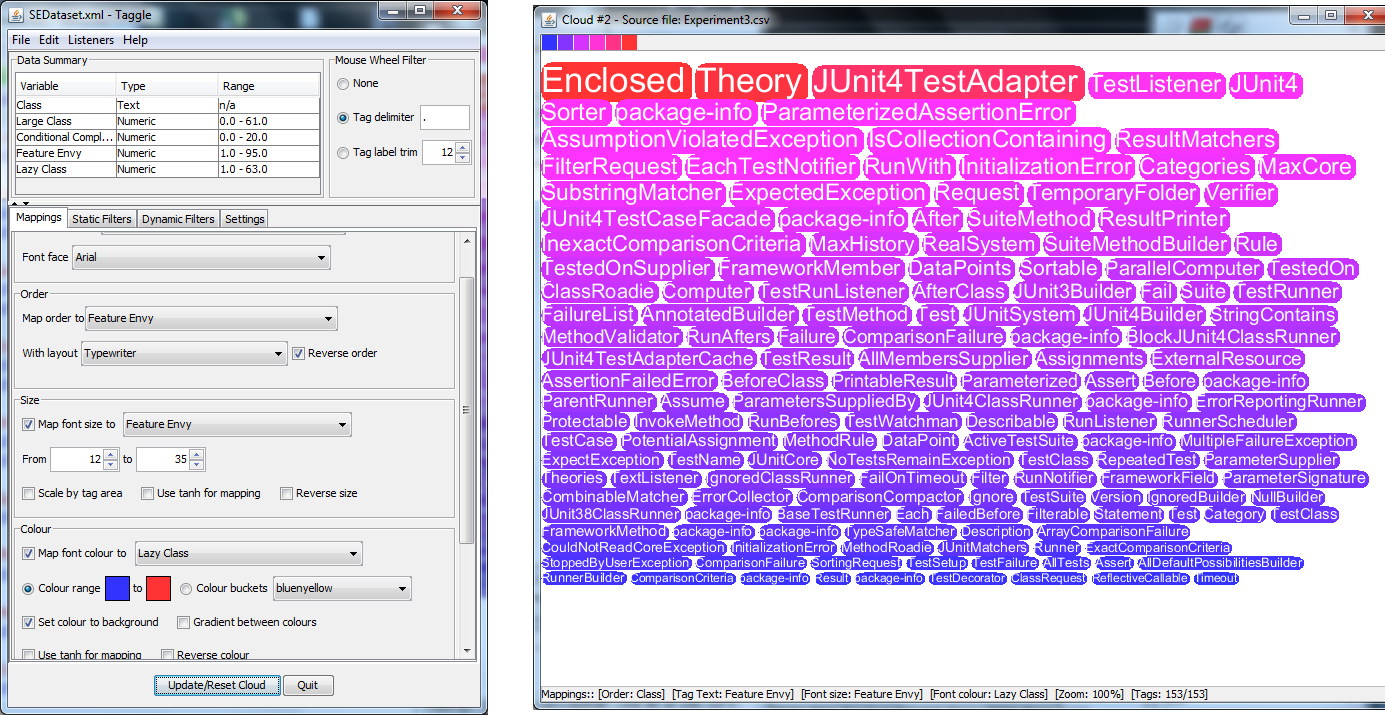
\includegraphics[scale=0.45]{correlation.png}
	\caption{\emph{Popularity ranking and composer date of death}}
	\label{fig:tagcorrelation}
\end{figure}

\section{Summary and discussion}

The design considerations for an interactive tag cloud visualisation tool presented in this chapter have been developed through analysis of current tag cloud and information visualisation research, guidelines, and principles. We summarise these considerations in Table~\ref{tab:designconsiderations}.

\begin{longtable}{|p{5cm}|p{9cm}|} 
%\caption{\textit{Design considerations for an interactive tag cloud tool}}
\hline
\textbf{Design Considerations} & \textbf{Description} \\
\hline
\endfirsthead
\multicolumn{2}{c}%
{\tablename\ \thetable\ -- \textit{Continued from previous page}} \\
\hline
\textbf{Design Considerations} & \textbf{Description} \\
\hline
\endhead
%\hline 

\multicolumn{2}{r}{\textit{Continued on next page}} \\
\endfoot
\hline
\endlastfoot
Textual datasets & Optimal datasets contain textual identifiers such as class names or stories.\\
Filterable tag phrases & Multiple words waste valuable real estate in a visualisation, so should be filterable.\\
Establish tag boundaries & Boundaries between tags with multiple words should be clearly established.\\
Tag order & Visual property tag order is suitable for mapping to data fields.\\
Equal length tag identifiers & It should be possible to set the length of the tag identifiers to an equal length to minimise effects on user perception.\\
Font size & Visual property tag order is suitable for mapping to data fields.\\	
Constrained font sizes & Font size should be constrained to greater than 9pt, and a suitable maximum font size according to canvas and screen boundaries.\\
Comparable tags & Tags should be able to be compared by moving closer together to assist quantitative comparisons.\\
Font family & Visual property tag order is not suitable for mapping to data fields.\\	
Familiar fonts & For reading accuracy, fonts should be familiar such as Times New Roman, Arial or Helvetica.\\	
Colour hue & Visual property colour hue is suitable for mapping to data fields.\\	
Colour transparency & Visual property colour transparency is suitable for mapping to data fields.\\	
Colour selection & Colour codes should be taken from Ware's  colour code recommendations (red, green, yellow, black, blue, white, pink, cyan, grey, orange, brown, and purple).\\	
Colour background & Visual property colour background is suitable for mapping to data fields.\\	
Colour contrasts & Strongly contrasting colour schemes should be selected such as red, blue and green on a white background.\\	
Font styles & Visual property font styles are not considered suitable for mapping to data fields.
\label{tab:designconsiderations}
\end{longtable}


In \S\ref{sect:tasktypes}, we presented a set of task types that we believe should be supported in a tag cloud visualisation tool in order to enable exploration of a software engineering dataset. These task types were generated from analysing software visualisation challenges and tag cloud capabilities. The task types and design considerations were used to inform the design of our interactive tag cloud visualisation system `Taggle', presented in Chapter~\ref{chap:taggle}.
	
% ------------------------------------------------------------------------


%%% Local Variables: 
%%% mode: latex
%%% TeX-master: "../thesis"
%%% End: 
